\chapter{XAI}\label{chapter:xai}

In his book "Interpretable Machine Learning" \parencite{molnar2022} Molnar describes the fundamentals of \ac{XAI}. This chapter is based on Molnar's findings. The idea behind \ac{XAI} is to be able to explain decisions made by an Artificial Intelligence, or \ac{ML} model. The ability to understand the underlying model's decisions can be crucial for real world applications of \ac{ML} models. One goal of \ac{XAI} is to increase the social acceptance of models by giving insights into why a model has made a certain decision. For example, in the application of self-driving cars, in the case of an accident, it is useful to understand why the car has made the decisions it has made and possibly even prove that the behavior prior to the accident was correct.
\\\\
For the case of this thesis, the goal of applying \ac{XAI} to the trained \ac{ML} models is to be able to understand which optimizations benefit from which configurations. 

\section{Characteristics of XAI techniques}
Since the topic of \ac{XAI} covers numerous algorithms, their characteristics can be broken down into whether a technique is \textbf{model-agnostic} or \textbf{model-specific} and whether it is a \textbf{local} or \textbf{global} explanation. The figure \ref{fig:xaioverview} provides an overview of these characteristics and how they relate to each other. 
\begin{figure}[h]
      \centering
      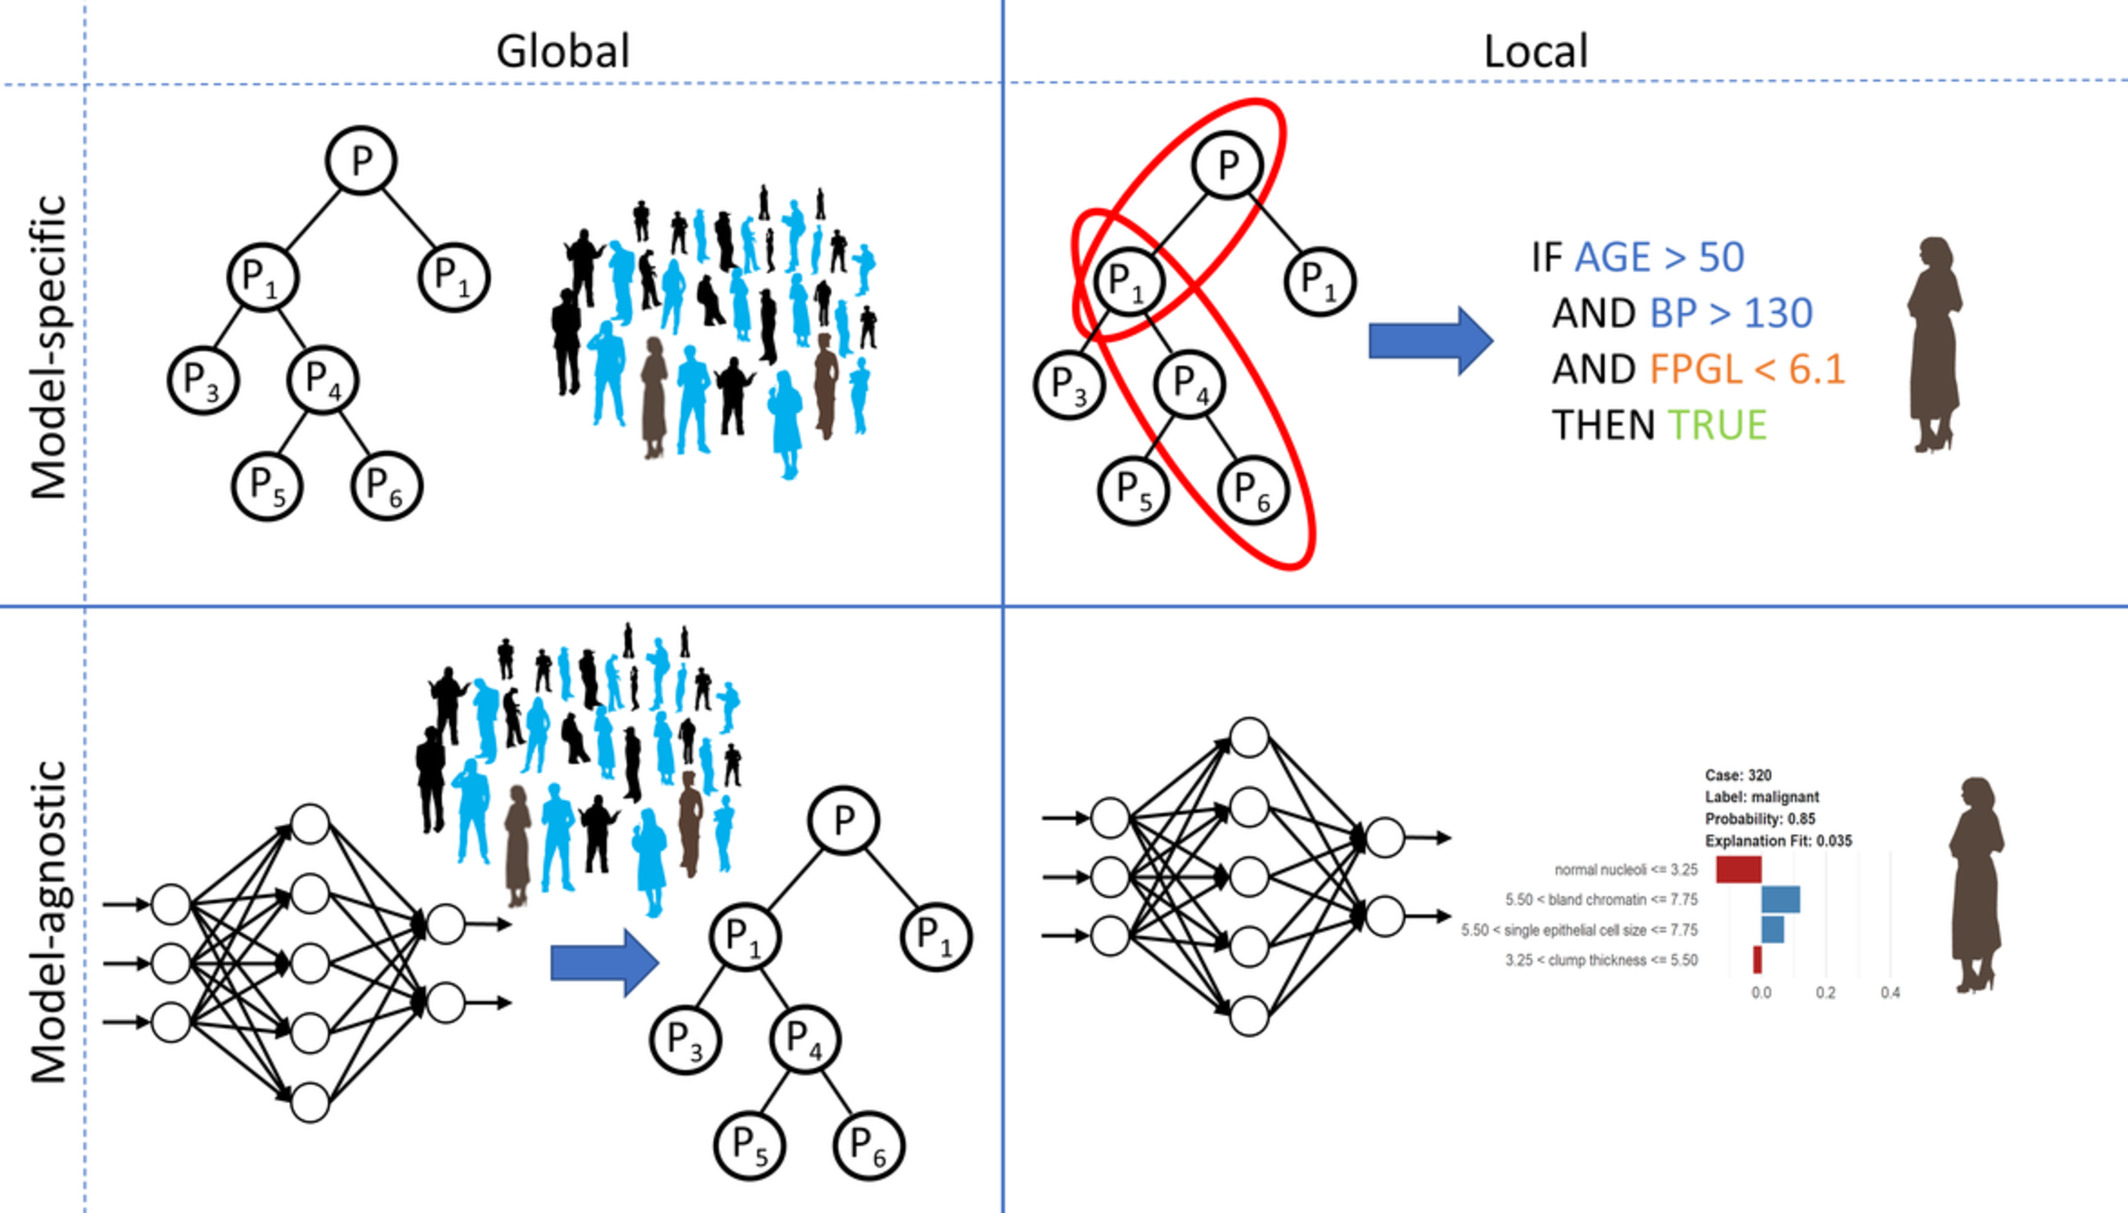
\includegraphics[width=0.8\textwidth]{images/XAI_overview.jpg}
      \caption{Overview of characteristics of XAI techniques \parencite{xaioverview}}
      \label{fig:xaioverview}
  \end{figure}
\\\
\textbf{Model-agnostic vs. model-specific}: Model-agnostic refers to techniques that can be applied to any \ac{ML} models. They consider the models as a black-box, meaning that they analyze the relationship between the inputs and the outputs and do not look deeper into the internal functionality of the models. Model-specific techniques are able to analyze the internal functionality of the models, but are limited to a specific type of models. These type of models can for example explain the weights of a linear model, or interpret the nodes in a neural network. 
\\\\
\textbf{Local vs. global}: Local \ac{XAI} techniques focus on interpreting the results of individual values, while global techniques interpret the model as a whole. Local techniques are not further discussed in this thesis, since interpreting individual runs of the benchmarking program does not provide a general picture about B+ tree configurations. They are more useful for real-world applications, where individual model decisions need to be explained. 
\\\\
\textbf{Model transparency}: Some machine learning models are considered transparent, or white-box, which refers to the interpretable nature of the model itself. Transparent models are considered to be easily humanly interpretable. A common case for this is a decision tree model, which is also used in figure \ref{fig:xaioverview} to represent explainable models. Not all transparent models are necessarily easily interpretable. For example, in the case of a decision tree model, if the tree has a big depth, the interpretations, can get incomprehensible. Linear models can be globally and locally explained, by analyzing the feature weights, however, there is the assumption that all features are statistically independent of each other.
\\\\
Out of the numerous algorithms that are part of \ac{XAI}, this thesis focuses on the algorithms that are suited for the use-case of this thesis. Model-specific interpretations are covered in the chapter \ref{chapter:findings}. It should be noted that the mathematical background of the individual algorithms is out of the scope of this thesis. Instead, this thesis aims to explain core ideas, the advantages, and disadvantages of the techniques.

\section{Permutation Feature Importance}
Permutation feature importance is a global model-agnostic method. The goal of this method is to identify, which features are important and which are less relevant. This is done by shuffling values of individual features and measuring the error of the model. One example of a permutation feature importance output, provided by the \textit{scikit-learn} implementation \parencite{42Permut82:online} used in this thesis, is presented in figure \ref{fig:permimp}. The plot highlights that the features \textit{sex}, \textit{pclass} and \textit{age} have the highest importance on an example model. Since various permutations are tested per feature, a box plot represents the output. 

\begin{figure}[H]
      \centering
      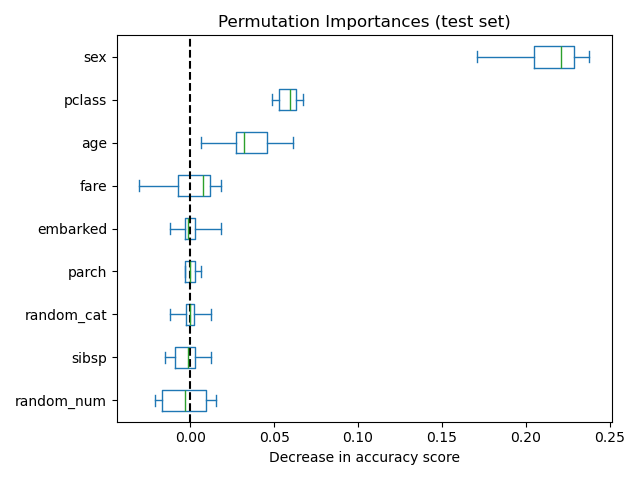
\includegraphics[width=0.5\textwidth]{images/feature_importance.png}
      \caption{Example output for permutation feature importance \parencite{42Permut82:online}}
      \label{fig:permimp}
  \end{figure}

\section{SHAP - SHapley Additive exPlanations}
SHAP is a technique that at its core is a local model-agnostic method. The idea behind this method is that a single record can be taken, and an individual feature is permuted to identify how the permutation impacts the result. The importance is measured in a so-called \textit{Shapley value}. KernelSHAP \parencite{shapKern53:online} is an algorithm used in this thesis, which trains a special weighted linear regression model to calculate the Shapley values of a record. For this thesis, however, local explanations are not relevant. \\
Nevertheless, KernelSHAP is used in this thesis, since applying the algorithm on multiple samples and plotting them in a \textbf{SHAP summary plot}, can give a broader, global picture about a model. An example for such a plot is given in figure \ref{fig:shapfeatimp}. This plot is beeswarm plot, where each dot represents a Shapley value of a record for each feature. The color of a dot indicates the value of a feature of a record from low to high. The density of the dots is visualized by stacking dots along the y-axis. The features are sorted from the highest mean of absolute Shapley values to the lowest.
\\\\
One can compare the SHAP summary plot to the permutation feature importance. They both intend to outline the feature importance, however the difference lies in the underlying structure of the algorithms. Permutation feature importance calculates the error by permuting features for all values, while SHAP feature importance takes the average impacts of features for individual values.

\begin{figure}[H]
      \centering
      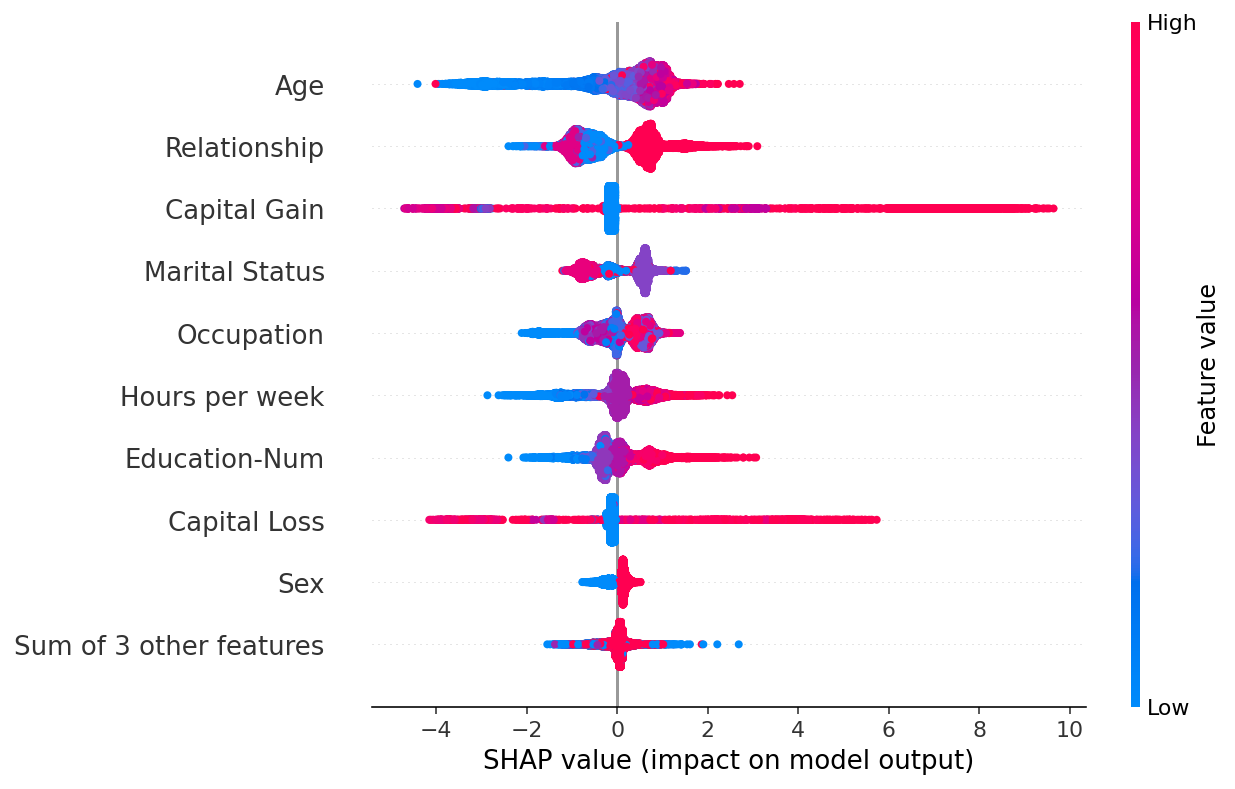
\includegraphics[width=0.7\textwidth]{images/SHAP_example.png}
      \caption{Example output for SHAP feature importance \parencite{barplot—98:online}}
      \label{fig:shapfeatimp}
  \end{figure}
